% \mychapter{Results and Discussion}{cap:results}
% \lhead{RESULTS AND DISCUSSION}

% %\section{Results}\label{sec:results}  

% In this chapter, we evaluate and compare the proposed model (COMP), which was implemented with the IBM ILOG CPLEX Optimization Studio v12.5.0 solver and executed on a computer Intel Core i5-6200U (2.30GHz and 4 cores) with 4GB of RAM, Ubuntu 16.04 LTS operating system. Our experiments are resumed as follows.  In Sec. \ref{sec:result:time}, we analyze the influence of weight values changing (weights of linear scalarization method) on CPU time. In Sec. \ref{sec:result:allocation}, we measure the quality of a feasible allocation obtained from the simulation approach. Finally, in Sec. \ref{sec:result:bandwidght}, we evaluate the performance of the proposed allocation process in terms of bandwidth availability management.

% The initial results of our model were published and are available in \citep{ramos:2019} and \citep{ramossbpo:2019} . The (COMP) model composed with Equation \eqref{equ:users2} and the heuristic method will be evaluated and discussed in future results.


% \section{Execution Time}
% \label{sec:result:time}

% Table \ref{tbl:exetime} shows the average execution time for different combinations of the weights $w_1$, $w_2$ and $w_3$. For this test case, we considered 10 data centers and a sample of 60 base stations in the city of Maceió, Alagoas, available in Telebrasil's database, which has latitude and longitude data of several base stations of different carriers in Brazil. Ten users are randomly placed and maintained in positions near eNBs so that the model can calculate distances. Since handover data and communication costs between data centers and eNBs are not available, we generated 30 instances of these values for each eNB, also randomly. We compute the execution time for every single instance, and in the end, we calculate the average execution time for the different weight combinations.

% \begin{table}[!htb]
%     \centering
%     \begin{tabular}{|c|c|c|c|}
%         \hline
%         $w_1$  & $w_2$  & $w_3$  & Average execution time (seconds) \\ \hline
%         1   & 0   & 0   & 0.75                               \\
%         0   & 1   & 0   & 1.09                               \\
%         0   & 0   & 1   & 1.13                               \\
%         0.8 & 0.1 & 0.1 & 2.04                               \\
%         0.1 & 0.8 & 0.1 & 4.44                               \\
%         0.1 & 0.1 & 0.8 & 2.42                               \\
%         0.4 & 0.3 & 0.3 & 2.69                               \\
%         0.3 & 0.4 & 0.3 & 2.70                               \\
%         0.3 & 0.3 & 0.4 & 2.42                               \\
%         0.9 & 0.1 & 0   & 1.69                               \\
%         0.1 & 0.9 & 0   & 4.17                               \\ \hline
%     \end{tabular}
%     \caption{Average execution time for different weights combinations. Total number of instances = 30, $N$ = 60, $DC$ = 10, $U$ = 10.}
%     \label{tbl:exetime}
% \end{table}

% In the the formulation (COMP), the weight configurations $(1, 0, 0)$, $(0, 1, 0)$ and $(0, 0, 1)$  verify the execution time in an isolated manner for $f(x_{ij}, h_{ij})$, $g(c_{is}, y_{is})$ and $z(b_{ki}, d_{ki}, \overline{h_i})$, since only one of the three criteria is considered. In a case of assigning higher priority to a specific criterion, it is observable that the execution time increases considerably for the weights combination $(0.1, 0.8, 0.1)$, which is when the costs of communication between eNBs and data centers need to be strictly optimized. If an approximately uniform combination such as $(0.4, 0.3, 0.3)$, $(0.3, 0.4, 0.3)$ or $(0.3, 0.3, 0.4)$ is to be taken, the average execution times are similar. We can verify Taleb et al. \cite{tarik2015} base model average execution time by making $z(b_{ki}, d_{ki}, \overline{h_i}) = 0$, which results in Eq. \eqref{equ:fo-mult}. Configuration $(0.1, 0.9, 0)$ shows that it takes longer to find an optimized solution to minimized communication costs with high priority, and low priority for reduced number of handover between coverage areas. In the opposite case, $(0.9, 0.1, 0)$, a considerable smaller average execution time is required.

% \section{User allocation}
% \label{sec:result:allocation}

% We collected latitude and longitude data from the Google Maps location history of a moving UE. Fig. \ref{fig:uecoords} shows the starting point of a 13.7 km displacement, traversed in a time interval of 42 minutes. The user followed the path from the starting point to the highest-numbered base station (21 in total), some of them illustrated by Fig. \ref{fig:enbcoords}. We found several base station locations in the database provided by \cite{telebrasil:2019}. In this study case, for every new UE's location, the model must evaluate if it is worth keeping it allocated in the same eNB or if it is better to transfer it to another one. Haversine Eq.~\eqref{equ:haversin} gives the distance between user and base station in this scenario.

% \begin{figure}[!htb]
% \centering
%     \subfigure[eNBs placement along the path traveled by UE.]{\label{fig:uecoords}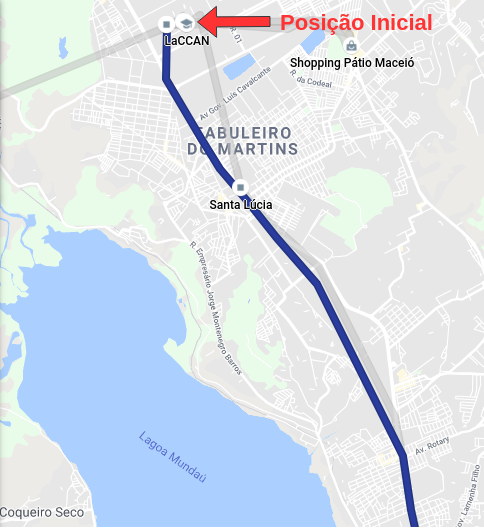
\includegraphics[width=.45\linewidth, height=8cm]{img/uecoords.png}}
%     \subfigure[eNBs in which the UE was allocated over the path.]{\label{fig:enbcoords}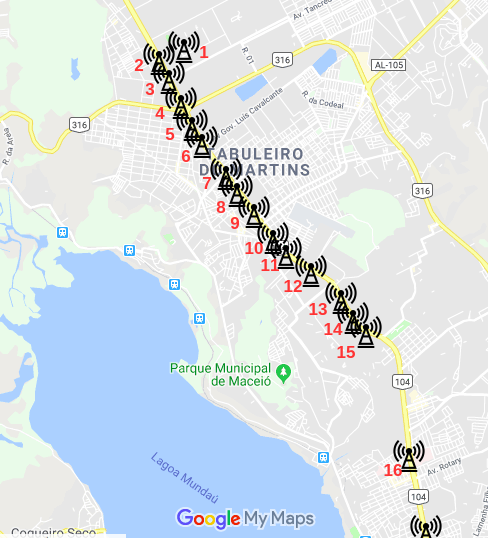
\includegraphics[width=.45\linewidth, height=8cm]{img/enbscoords.png}}
%     \caption{Path traveled by UE over time, moving forward from the starting point to the highest-numbered eNB.}
% \end{figure}

% Fig. \ref{fig:enbplot2} shows the eNBs where the system allocates the UE over the 13.7 km path. According to its GPS information, the initial UE position was nearby eNB$_1$ and eNB$_2$, with respective distances of 0.08 km and 0.45 km. The average handover of these base stations is 5.3 for the first and 3.75 for the second. The formulation (COMP) allocates UEs in eNBs with the smallest sum of distance and handover average, thus, it is observable in Fig. \ref{fig:enbplot2} the correct allocation in eNB$_2$. During the last 10 minutes of the traveled path, eNB$_{19}$, eNB$_{20}$ and eNB$_{21}$ are closer, at a respective distance of 0.78, 0.91 and 0.53 kilometers. Their handover averages are 3.8, 6.25, 5.5, which causes the permanence of UE in eNB$_{19}$.

% \begin{figure}[!htb]
%     \centering
%     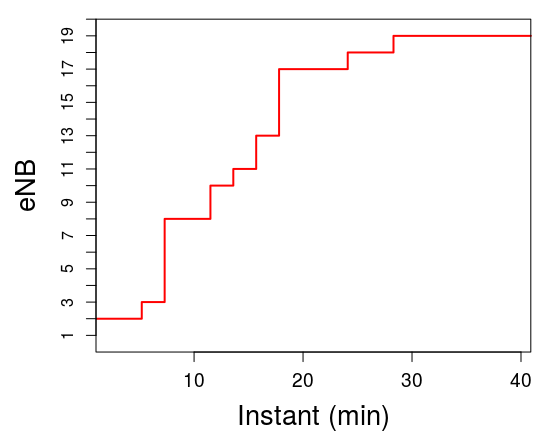
\includegraphics[width=.65\linewidth]{img/enbplot2.png}
%     \caption{eNB in which the UE was allocated over the travel time.}
%     \label{fig:enbplot2}
% \end{figure}

% \section{Bandwidth Management}
% \label{sec:result:bandwidght}

% To evaluate the model (COMP) bandwidth management, we simulated a second mobility scenario with 20 UEs and 5 eNBs. The bandwidth restrictions for eNBs and UEs are respectively $L_i$ = 20 Mbps and $l_k$ = 3 Mbps (hypothetical values). The model does not have time as a direct parameter, but the position (which influences the value of $d_{ki}$) changes over time. In this test case, UE's position $x$ is given by the function $x = t$, and $t$ represents a time instant. As previously illustrated in the flowchart of Fig. \ref{fig:flowchart}, the model is executed periodically, at a instant $t$. The graph in Fig. \ref{fig:ueposXenb} shows the base station that an user (namely UE$_1$) has been allocated. From the moment it becomes very costly to remain connected to a base station (because of distance or eNB handover average), e. g., eNB$_1$, the system will transfer the user to another eNB, Fig \ref{fig:ueposXenb}. The transition from eNB$_1$ to eNB$_2$ is performed near position $x = 30$.

% \begin{figure}[!htb]
%     \centering
%     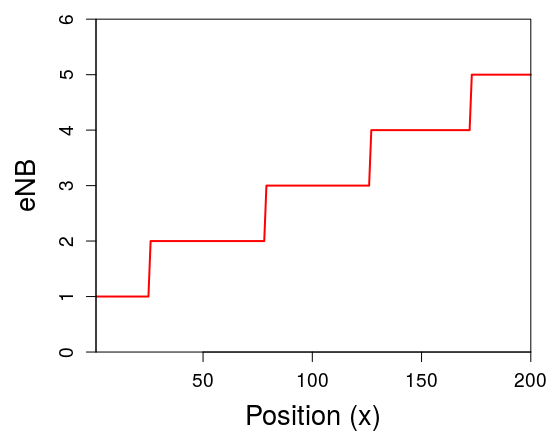
\includegraphics[width=.65\linewidth]{img/plot_ueposXenb.png}
%     \caption{eNB$_i$ in which $UE_1$ is allocated according to its position.}
%     \label{fig:ueposXenb}
% \end{figure}

% The process repeats as UE$_1$ moves towards other base stations. The remaining 19 UEs are not moving so we can easily see the behavior of the network. The graphs in Fig. \ref{fig:enbues} and \ref{fig:enbbdw} show respectively the number of UEs allocated and the available bandwidth in each eNB, which changes as UE$_1$ is transferred between eNBs. We can see in Fig. \ref{fig:enbues} that eNB$_1$ initially has 2 connected UEs. It is also known that UE$_1$ has its position determined by $x = t$. Therefore, at $t = 0$, UE$_1$ is at $x = 0$ and allocated in eNB$_1$. Observing the bandwidth availability of eNB$_1$ in Fig. \ref{fig:enbbdw} at $t = 0$, for 2 connected users with minimum requirements of 3 Mbps, it is verifiable that the base station has only 14 Mbps, from a total $L_1$ = 20 Mbps.

% \begin{figure}[!htb]
%     \centering
%     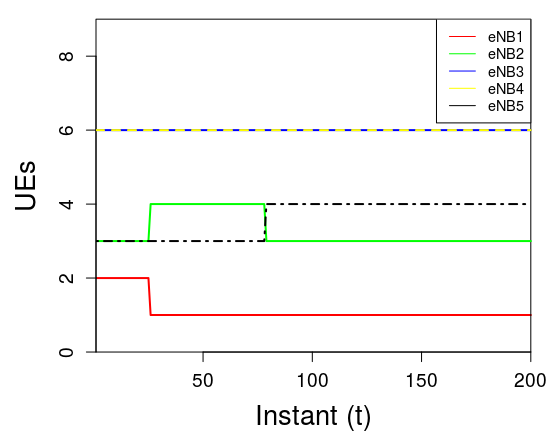
\includegraphics[width=.65\linewidth]{img/plot_tXues.png}
%     \caption{Number of connected UEs in each eNB over time.}
%     \label{fig:enbues}
% \end{figure}

% \begin{figure}[!htb]
%     \centering
%     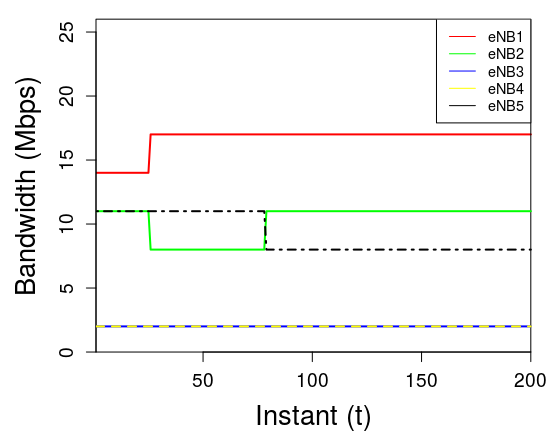
\includegraphics[width=.65\linewidth]{img/plot_tXbdw.png}
%     \caption{Available bandwidth in each eNB at instant t.}
%     \label{fig:enbbdw}
% \end{figure}

% The rearrangement of the network can be verified as UE$_1$ moves. As previously shown, the transfer of eNB$_1$ to eNB$_2$ occurs approximately at $x = 30$. We can see the change in the number of UEs in eNB$_1$ (from 2 to 1) and eNB$_2$ (from 3 to 4) in Fig. \ref{fig:enbues} at $t \approx 30$. The gain or loss of available bandwidth is observable in Fig. \ref{fig:enbbdw} at the same instant $t$. Since eNB$_4$ and eNB$_5$ are always operating with 6 users, their bandwidth availability is low and not enough to serve another UE. However, when approaching these base stations, UE$_1$ will certainly connect to them, as is observable in Fig \ref{fig:enbues}. This behavior is possible because even if operating in full capacity, the network will rearrange UEs in different eNBs, ensuring that each of them has a base station connection.